\documentclass[10pt,twocolumn,letterpaper]{article}

\usepackage{cvpr}
\usepackage{times}
\usepackage{epsfig}
\usepackage[utf8]{inputenc}
\usepackage{graphicx}
\usepackage{refstyle}
\usepackage{amsmath}
\usepackage{amssymb}
\usepackage{algpseudocode}
\usepackage{algorithm}
\usepackage{booktabs}
\usepackage{pbox}
\usepackage{cite}

% Include other packages here, before hyperref.

% If you comment hyperref and then uncomment it, you should delete
% egpaper.aux before re-running latex.  (Or just hit 'q' on the first latex
% run, let it finish, and you should be clear).
\usepackage[breaklinks=true,bookmarks=false]{hyperref}

\cvprfinalcopy % *** Uncomment this line for the final submission

\def\cvprPaperID{****} % *** Enter the CVPR Paper ID here
\def\httilde{\mbox{\tt\raisebox{-.5ex}{\symbol{126}}}}

% Pages are numbered in submission mode, and unnumbered in camera-ready
%\ifcvprfinal\pagestyle{empty}\fi
\setcounter{page}{1}
\begin{document}

%%%%%%%%% TITLE
\title{Investigation of Different Filters Based on Gesture Recognition System}

\author{Chen Du\\
PID: A53223649\\
{\tt\small c9du@eng.ucsd.edu}
% For a paper whose authors are all at the same institution,
% omit the following lines up until the closing ``}''.
% Additional authors and addresses can be added with ``\and'',
% just like the second author.
% To save space, use either the email address or home page, not both
\and
Wenjun Zhang\\
PID: A53218995\\
{\tt\small wez177@eng.ucsd.edu}
\and
Jingyi Yang\\
PID: A53216941\\
{\tt\small jiy349@eng.ucsd.edu}
\and
Jinzhao Feng\\
PID: \\
{\tt\small @eng.ucsd.edu}
}

\maketitle
%\thispagestyle{empty}

%%%%%%%%% ABSTRACT
\begin{abstract}
Gesture recognition is an important task of modern Computer Vision, which has been widely used in human-computer interaction, game industry and internet of things. A big challenge in gesture recognition is the high precision tracking of fingers and hand. Many filter algorithms has been proposed for object tracking with different characterizations. Given correct motion model, Unscented Kalman Filter is one of the best choice. In this project, we build a gesture recognition system which could identify simple number gestures, and implement four kinds of filter algorithms to investigate their performances in different scenarios. Results show that Unscented Kalman Filter has overall best performance and robustness, and particle filter with enough particles also has great tracking precision without interference.
\end{abstract}

%%%%%%%%% BODY TEXT
\section{Introduction}

Gestures are naturally performed by human-being. Produced as a part of deliberate actions, signs or subconscious intentions and attitude, hand gestures are essential in communication, which has been the focus of studies. Gestures are present in most daily human actions and participate in human communication by either complementing speech or substituting themselves to spoken language in environments requiring silent communication (under water, noisy environments, secret communication,
etc.) or for people with hearing disabilities.\cite{ref:escalera}

Given the indubitable importance of gestures in human activities, there has been huge interest from the Computer Vision and Machine Learning communities to analyze human gestures from visual data in order to offer new non-intrusive technological solutions.  In particular, interfaces incorporating hand gestures have gained popularity\cite{ref:ohn} in automobile industry. For example, BMW has applied gesture recognition in their newest iDrive system so as to control the vehicle's navigation, buttons, knobs, windows and voice commands. Moreover, depth cameras have been widely utilized in camera tracking for augmented and mixed reality\cite{ref:otto}, as well as popular games such as Just Dance from Ubisoft.

To capture the meaning of the gesture, finger tracking is the fundamental part. Many tracking techniques are available in object tracking. For example, the Kalman Filter, which has been introduced decades ago, and its corresponding improvements, the Extended Kalman Filter and Unscented Kalman Filter, which are used to deal with nonlinear problems. Also, the Particle Filter, which is usually applied with color detection in object tracking. However, each technique is of their own strengths and weakness, under different scenarios, their performance may differ. An obvious way to determine the performance is by visually comparing the object and trajectory. But a more convincing way is to set the ground truth of the object and compute the precision statistically.

In this article, we introduce a self-built gesture recognition system with MATLAB programming, and implement Kalman, Extended Kalman, Unscented Kalman and Particles filters with different parameters for object tracking and gesture recognition. We investigate their performance statistically under different scenarios, including linear motion, nonlinear motion, motion with object being occluded and circumstance in low light.

Identifying an object in a real-world environment is of great difference from tracking the detection of the object. In this article we mostly focus on the tracking of already identified objects rather than the method of how to detect the object. The structure of the paper consists of 4 parts: first we provide a brief description of the gesture recognition system we build, followed by the theory introduction of the filters we applied in the system. Next, we provide the experiments that we implemented for the comparison of the filters' performance. Finally, we draw conclusion based on the results of the experiments.

%------------------------------------------------------------------------
\section{Gesture Recognition System}

We built our gesture recognition system which could recognize number gesture from one to five and show the corresponding numbers. This system is based on Matlab, which is one of the most popular computer vision platforms. The block diagram of the system is shown in Figure \ref{fig: system diagram}. This system could be separate into 3 parts: detection, tracking and recognition.

\begin{figure}[h]
     \centering
       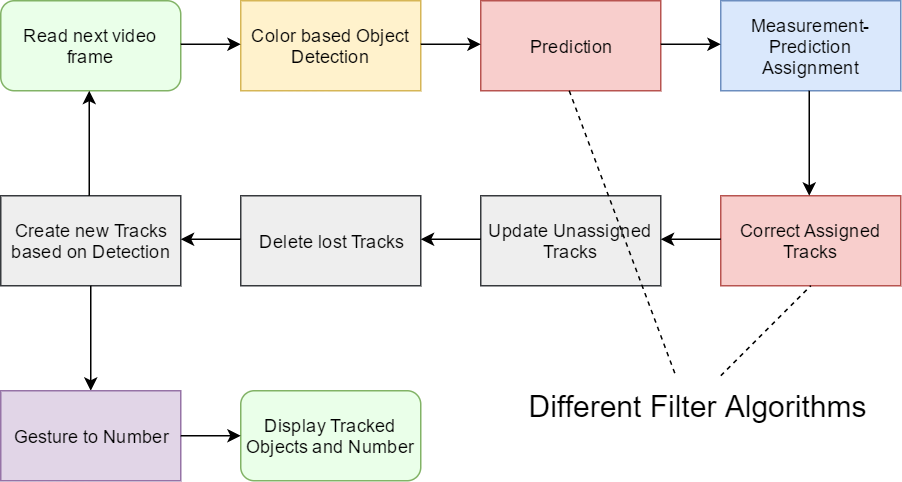
\includegraphics[width=0.5\textwidth]{duchen_1.png}
         \caption{\small{Diagram of Gesture Recognition System}}
         \label{fig: system diagram}
 \end{figure}

\subsection{Object Detection}

We have tested 3 detection methods including correlation bases detection \cite{ref:kernel}, foreground detection \cite{ref:gallego2009} and color-based detection \cite{ref:khan2001object}. Since the correlation-based object detection needs a specific template for each object and is unstable when object or lens rotates, it appeared low precision for finger detection where lots of rotations and random motions happen. Similarly, the foreground detection has a demand for fixed camera, and is hard to tell the fingers from non-target moving objects interference. Color-based detection is widely used in scenes where the objects have specific color, and has the advantage of robustness for moving object detection compared with other two methods. Using a glove with specific colored fingers, the color-based detection showed high precision and robustness. So we choose the color-based object detection to capture the fingers and hand locations. In detail, in each frame, the RGB value of each pixel $<r_x, g_x, b_x>$ is compared with the target RGB value $<r_t, g_t, b_t>$, and the Euclidean norm of the difference is calculated as the distance:

\begin{equation}
dist_x=||r_x-r_t||+||g_x-g_t||+||b_x-b_t||\\
\end{equation}

If the distance is within a given threshold $dist_{th}$, this pixel is judged as target (foreground).

\begin{equation}
	target_x=
\begin{cases}
	1, & dist_x<dist_{th}\\
	0, & dist_x>dist_{th}
\end{cases}
\end{equation}

A mask of target is formed after all pixels have been judged. A blob analysis is performed on the mask and the finger-like connected components within given size will be output as the fingers and the centers are calculated as locations. Before blob analysis, we remove small connected components within a given area threshold (e.g. 100 pixels) to prevent false positive, then a morphologic closing is applied to remove the false negative holes caused by noise.

\subsection{Tracking}
We applied 4 kinds of filters which will be discussed in section 3. For multiple object tracking, one challenge is to correctly assign the predicted locations with the detected ones. Here we use the state-space distance \cite{ref:welch1995introduction} to compute the confidence.

\begin{equation}
d(z)=(z-Hx)^T\sum^{-1} (z-Hx)+ln|\Sigma|
\end{equation}

\begin{equation}
\Sigma=HPH^T+R
\end{equation}

In the above equations, $z$ is the measurement and $d(z)$ is the corresponding state-space distance, $x$ is the predicted state, $P$ is the state estimation error covariance, $H$ is the measurement model, where all these metrics will be discussed in section 3. For each predicted state, we assign it to the measurement with lowest distance. For Kalman filters the assigned trackers will be corrected to get the tracked locations, while the unassigned trackers will just use predicted states as the tracked locations. For trackers which are unassigned for a certain number of continuous frames, we regard them as lost objects and delete them. For unassigned measurements new trackers will be created once they show up longer than a certain number of continuous frames.

\subsection{Convert Gesture to Number}

Once we have the tracked locations of the fingers and hand, we establish a 3x3 grid block based on hand location and count the finger numbers in each block, then output the corresponding meaning of the gesture, here the output contains numbers from 1-5. The connection between number count and the output is set manually, and is adjustable to add other meanings of gestures.

\begin{figure}[h]
     \centering
       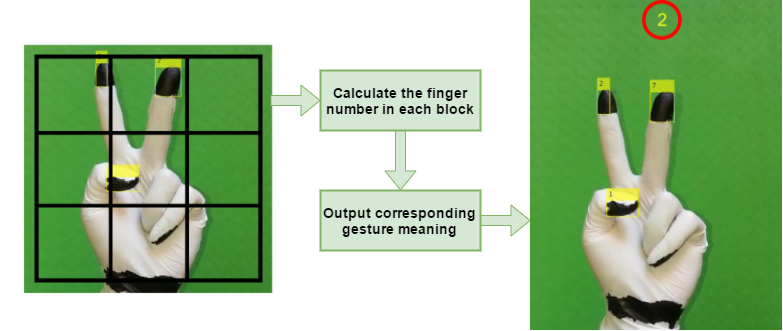
\includegraphics[width=0.5\textwidth]{duchen_2.png}
         \caption{\small{Gesture-to-number Conversion}}
         \label{fig: conversion}
 \end{figure}

%------------------------------------------------------------------------
\section{Filter Theory}

\subsection{Kalman Filter}

Kalman filter has been widely applied in object tracking. The Kalman filter is the optimal filter to estimate the state of a linear dynamic system when only noisy measurements are available\cite{ref:botond2008}. Due to analytic tractability both operation and measurement noises are required to be Gaussian. In 1960, Ruodolf Kalman first introduced the system\cite{ref:kalman}, and it was first applied in estimating the trajectory for the NASA Apollo program in 1969\cite{ref:grewal}.

The operation of the filter basically consists of 2 steps:

1. Prediction, based on the last estimated state $\hat{x}_{k-1}$ and covariance matrix $P_{k-1}$:

\begin{equation}
\hat{x}_k^-=A\hat{x}_{k-1}+Bu_k
\end{equation}

\begin{equation}
P_k^-=AP_{k-1}A^T+Q
\end{equation}

where $A$ is the time-transition matrix,  $u_k$ is the control or external input, $B$ is a linear matrix which characterize the effects of the external input, and $Q$ is the operation noise covariance matrix.

Equation (5) predicts the most probable state $\hat{x}_k^-$ based on the last estimation and the external input. Equation (6) predicts the new covariance matrix $P_k^-$ of the predicted state, given the previous estimated covariance matrix and operation noise.

2. Correction, based on the measurements to correct the prediction:

\begin{equation}
K_k=P_k^-H^T(HP_k^-H^T+R)^{-1}
\end{equation}

\begin{equation}
\hat{x}_k=\hat{x}_k^-+K_k(z_k-H\hat{x}_k^-)
\end{equation}

\begin{equation}
P_k=(I-K_kH)P_k^-
\end{equation}

where $K_k$ is the Kalman gain, the term $z_k-H\hat{x}_k^-$ is called the innovation, $H$ is the measurement matrix, and $R$ is the measurement noise covariance matrix.

The Kalman gain $K_k$ controls the effect that the current measurement has over the new state. Equation (8) and (9) correct the prediction based on the Kalman gain to estimate the state $\hat{x}_k$ and covariance matrix $P_k$.

It should be noted that the transition matrix $A$ and measurement matrix H in Kalman filter are certain, so when the model is non-linear, no such certain matrices $A$ or $H$ exists, and Kalman filter no longer works.

%-------------------------------------------------------------------------
\subsection{Extended Kalman Filter}

The Extended Kalman filter (EKF)\cite{ref:peter}\cite{ref:sorenson} has been applied to alleviate the constraint of linearity. The basic framework of Extended Kalman filter is similar to that of Kalman filter, which is shown in Figure \ref{fig: EKF}.

\begin{figure}[h]
     \centering
       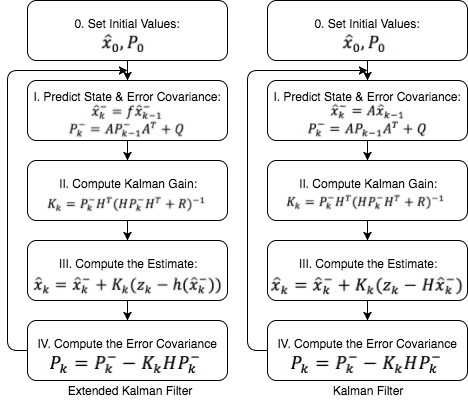
\includegraphics[width=0.5\textwidth]{EKF.png}
         \caption{\small{Diagram Comparison between EKF and KF}}
         \label{fig: EKF}
 \end{figure}
For convenience, the control input $u_k$ has been set to zero. The difference of the Extended Kalman filter are to use the nonlinear functions $f$ and $h$ for state and measurement prediction, and to substitute the transition matrix $A$ and measurement matrix $H$ with Jacobian matrices derived from the non-linear functions:

\begin{equation}
A=\frac{\partial f}{\partial x}|_{\hat{x}_{k-1}}
\end{equation}

\begin{equation}
H=\frac{\partial h}{\partial x}|_{\hat{x}_k^-}
\end{equation}

The Jacobian matrix is obtained through the first order partial derivative, so the Extended Kalman Filter can be viewed as "first order" approximation to the optimal terms[6]. However, the Extended Kalman filter can introduce large errors when the high order terms cannot be overlooked. As shown in Figure \ref{fig: mean and cov prop}\cite{ref:cyrill}, linearized transformation is not reliable if propagation cannot be well approximated by a linear function\cite{ref:ye}. In addition, linearization can be applied only if the Jacobian matrices exists. Furthermore, the heavy computation of Jacobian matrices makes EKF impractical in many situations.

\begin{figure}[h]
     \centering
       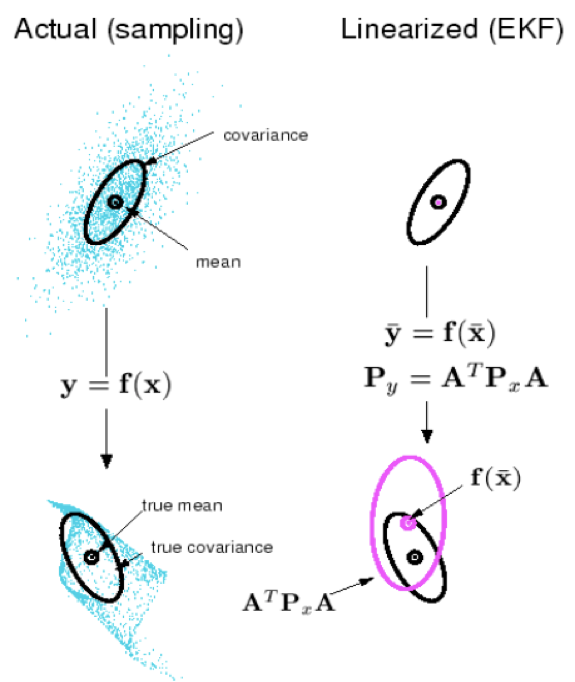
\includegraphics[width=0.4\textwidth]{pic_2.png}
        \caption{\small{Mean and Covariance Propagation}}
        \label{fig: mean and cov prop}
 \end{figure}

%-------------------------------------------------------------------------
\subsection{Unscented Kalman Filter}

The Unscented Kalman Filter\cite{ref:Julier} addresses the approximation issues of the Extended Kalman Filter. The intuition is to approximate a probability distribution rather than a non-linear function. To achieve this, a set of points are carefully chosen to described the mean and covariance, and the points are called the sigma points\cite{ref:ryan}.

The Unscented Kalman Filter can be seen as a combination of Unscented Transformation and Kalman Filter. We first start by explaining the unscented transformation\cite{ref:julierUhlmann}.

The unscented transformation(UT) is a method to compute the statistics of a random variable undergoing nonlinear transformation by transforming each sigma point through the nonlinear function. Suppose a random variable $x$ (dimension $n$) with mean $\mu$ and covariance matrix $
\sum$ is propagated through a nonlinear model with function $y=g(x)$. A matrix $X$ of $2n+1$ vectors $X_i$ is formed as the set of sigma points, and each vector is corresponding with weight $W_i$. The procedures are according to the following:

Choosing the sigma points

\begin{equation}
X^{[0]}=\mu
\end{equation}

\begin{equation}
X^{[i]}=\mu+(\sqrt{(n+\lambda)})_i\quad for \ i=1, ..., n
\end{equation}

\begin{equation}
X^{[i]}=\mu+(\sqrt{(n+\lambda)})_{i-n}\quad for \ i=n+1, ..., 2n
\end{equation}

Weights sigma points

\begin{equation}
w_m^{[0]}=\frac{\lambda}{n+\lambda}
\end{equation}

\begin{equation}
w_c^{[0]}=w_m^{[0]}+(1-\alpha^2+\beta)
\end{equation}

\begin{equation}
w_m^{[i]}=w_c^{[i]}=\frac{1}{2(n+\lambda)} \quad for \ i=1, ..., 2n
\end{equation}

where $\lambda=\alpha^2(n+k)-n$ is a scaling parameter. $\alpha$ is usually set to small value and $k$ is usually set to zero, and both of them determine how far the sigma points are away from the mean. $\beta$ is used to incorporate prior knowledge of the distribution of $x$, where $\beta=2$ is the optimal choice for Gaussians. $(\sqrt{(n+\lambda)})_i$ is the $i$ th row of the matrix square root. These sigma vectors are propagated through the nonlinear model,

\begin{equation}
Y_i=g(X_i) \quad for\  i=0, ..., 2n
\end{equation}

The mean and covariance of $y$ can be approximated by the summation of the weighted sample mean and covariance of the transformed sigma points,

\begin{equation}
\mu^{'}=\sum_{i=0}^{2n}w_m^{[i]}g(X^{[i]})
\end{equation}

\begin{equation}
\sum^{'}=\sum_{i=0}^{2n}w_c^{[i]}(g(X^{[i]})-\mu^{'})(g(X^{[i]})-\mu^{'})^T
\end{equation}

These sigma points completely capture the true mean and covariance accurately to the 3rd order for any nonlinearity. As shown in Figure \ref{fig: mean cov}\cite{ref:cyrill}, the right plots show the performance of the UT when using 5 sigma points, which outperforms the other two methods obviously.

\begin{figure}
     \centering
       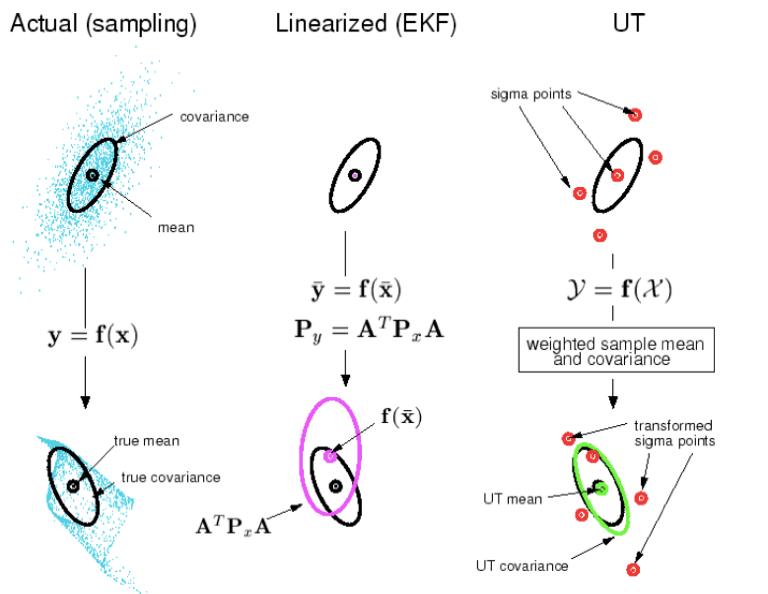
\includegraphics[width=0.5\textwidth]{pic_3.png}
        \caption{\small{Mean and Covariance Propagation}}
        \label{fig: mean cov}
 \end{figure}

Therefore, when the mean and covariance of the input are certain, the mean and covariance of the non-linear transformation can be computed using UT. The algorithm of Unscented Kalman Filter is shown in Algorithm 1: Unscented Kalman Filter Algorithm. The basic framework is the same as the Extended Kalman Filter. The difference is that, instead of using the nonlinear functions directly for prediction and the Jacobian matrices to linearize the model, the Unscented Kalman Filter applies the UT to obtain the mean and covariance of the nonlinear propagation\cite{ref:gustafsson}, so it does not require the computation of the Jacobian matrices.
\begin{algorithm}
\caption {Unscented Kalman Filter Algorithm}
\begin{algorithmic} [1]
\State  Unscented Kalman Filter$(\mu_{t-1},\quad \Sigma_{t-1},\quad u_t,\quad z_t)$
\State $\chi_{t-1}=(\mu_{t-1} \quad \mu_{t-1}+\sqrt{(n+\lambda)\Sigma_{t-1}} \quad \mu_{t-1}-\sqrt{(n+\lambda)\Sigma_{t-1}})$
\State $\bar\chi_t^*=g(u_t,\chi_{t-1})$
\State $\bar\mu_t=\sum_{i=0}^{2n} \omega_m^{[i]}\bar\chi_t^{*[i]}$
\State $\bar\Sigma_t=\sum_{i=0}^{2n} \omega_c^{[i]}(\bar\chi_t^{*[i]}-\bar\mu_t)(\bar\chi_t^{*[i]}-\bar\mu_t)^T+R_t$
\State $\bar\chi_t=(\bar\mu_t\quad \bar\mu_t+\sqrt{(n+\lambda)\bar\Sigma_t}\quad \bar\mu_t-\sqrt{(n+\lambda)\bar\Sigma_t})$
\State $\bar{Z}_t=h(\bar\chi_t)$
\State $\hat{z}_t=\sum_{i=0}^{2n} \omega_m^{[i]}\bar{Z}_t^{[i]}$
\State $S_t=\sum_{i=0}^{2n}  \omega_c^{[i]} (\bar{Z}_t^{[i]}-\hat{z}_t) (\bar{Z}_t^{[i]}-\hat{z}_t)^T+Q_t$
\State $\bar\Sigma_t^{x,z}=\sum_{i=0}^{2n} \omega_c^{[i]}(\bar\chi_t^{[i]}-\bar\mu_t)(\bar{Z}_t^{[i]}-\hat{z}_t)^T$
\State $K_t=\bar\Sigma_t^{x,z}S_t^{-1}$
\State $\mu_t=\bar\mu_t+K_t(z_t-\hat{z}_t)$
\State $\Sigma_t=\bar\Sigma_t-K_tS_tK_t^T$
\State $return\quad \mu_t,\Sigma_t$
\end{algorithmic}
\end{algorithm}

Though no Jacobian matrices are needed, the Unscented Kalman Filter belongs to the same complexity class with the Extended Kalman Filter. Besides, the Unscented Kalman Filter is still restricted to Gaussian distributions.

%-------------------------------------------------------------------------
\subsection{Particle Filter}

Another popular tool in object tracking is the Particle Filter\cite{ref:gordon}, which is also known as sequential Monte Carlo method\cite{ref:robert}. The Particle Filter method is an efficient method to apply simulation for estimating unknown probability distributions, and it is suitable in all kinds of frameworks, regardless of linearity and Gaussian. 

The basic idea of the algorithm is that any distribution can be represented as a set of weighted particle pairs $<x_k^{(i)}, w_k^{(i)}>$, where $x_k^{(i)}$ is a possible value of the system state and $w_k^{(i)}$ is its plausibility. Figure \ref{fig: particle} indicates the diagram of particle filter. In particle filtering a set of particle is first generated randomly to represent the initial distribution. The posterior distribution is defined by a new particle set and it's determined by a function $f$, which describes the dynamics of the system. The measurement update step is achieved by setting the weights according to the measurement data. The relation between the measurement data and the latent states is given by the conditional $h$. The most probably estimated state will be:

\begin{equation}
x_k=\sum_{i=1}x_k^{-(i)}w_k^{(i)}
\end{equation}

\begin{figure}[h]
     \centering
       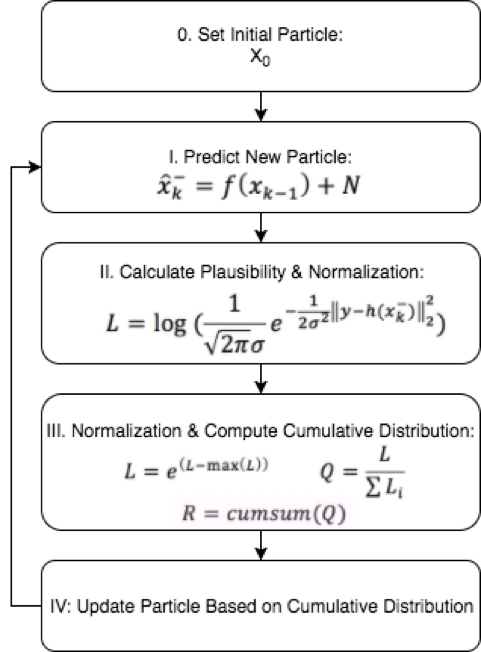
\includegraphics[width=0.3\textwidth]{pic_5.png}
        \caption{\small{Diagram of Particle Filter}}
        \label{fig: particle}
 \end{figure}

It frequently occurs that almost all weights are zero except for one which tends to be one when implementing the Particle Filter in its basic form. To eliminate the effect, the resampling\cite{ref:doucet} is very important. The distribution can be updated as the particles be resampled with the weights which we obtain from the measurement data, as shown in Figure \ref{fig: p resample}.

\begin{figure}[h]
     \centering
       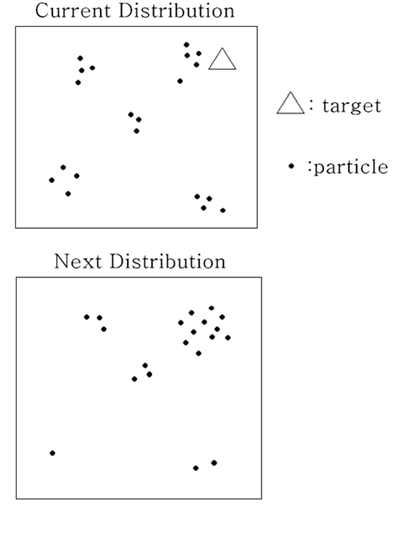
\includegraphics[width=0.5\textwidth]{Particle_Resampling.png}
        \caption{\small{Particles Resampling}}
        \label{fig: p resample}
 \end{figure}

When used in object tracking, the Particle Filter is usually applied with color detection and it is relatively easy to implement. However, since the information of a pixel is just RBG information, it cannot work for gray-scale video, and its precision decreases sharply for low-light and occluded objects. Another issue is the decision of the sample size for adequate performance. An efficient set size has been introduced by Kong and Liu\cite{ref:doucet}, which can be obtained from the weights of the particles following the equation below:

\begin{equation}
N_{eff}=\frac{N_s}{1+var(w_k)}
\end{equation}

where $N_s$ is the original set size. Notice that $N_{eff} \leq N_s$, and small $N_{eff}$ indicates severe degeneracy, which is an undesirable effect in particle filters. A direct way to reduce this effect is to use very large $N_s$. So sufficient amounts of particles are prerequisite to ensure accurate tracking, and it can require high computation load for large-size video.

%-------------------------------------------------------------------------
\section{Experiment Design and Results}

To investigate the performances of different filters and confirm the hypothesis, we use the detection and tracking parts of our system to do a quantitative evaluation experiment, which aims to compare the tracking using different filters in various scenarios.

\subsection{Scenario Selection}

Considering factors which could affect the tracking performances, we design and record videos in scenarios shown below:
1) Linear motion model: the objects perform simple linear motion, e.g. straight line motion. Note that there is no perfect linear motion in real life, so the linear motion is actually approximately linear motion. Despite small vibration or disturbance, the movement in a short period of continuous frame could be regarded as linear.
2) Nonlinear motion model: the objects perform mostly random motion, e.g. hand doing random gestures. It?s hard or impossible to manually calculate the state transition model in this case.
3) Occluded objects: objects are usually occluded in real life videos. A robust tracker should be able to handle the occlusion. In this kind of videos, objects are occluded partially or entirely in some frames, the occluded frame ratio varies from 10\% to 50\%.
4) Low-light condition: light is a very important factor that could influence the detection results. In this condition, objects moves in low-light environment which makes it hard to tell the target color for each pixel.
By choosing one of 2 motion models and one of 3 interferences (no interference is one choice), we have 6 combinations of scenarios.

\subsection{Evaluation Metric}

Many metrics for quantitative evaluation of target tracking have been proposed by researchers \cite{ref:bernardin2008evaluating}\cite{ref:li2009learning}\cite{ref:babenko2011robust}. Since we focus on the tracking performance comparison, the precision plot which is used in recent year tracking benchmarks \cite{ref:wu2013online}\cite{ref:wu2015object} is a suitable choice. The precision of a tracker means the percentage of frames whose estimated location is within the given threshold distance of the ground truth [8]. We are able to see the tracking performances with different error tolerances from precision plot directly.

\subsection{Parameters}

The system parameters are shown in Table 1, for different trackers and videos, the noise value is selected based on the scenario. When the detector works well, i.e. there is enough light and no occlusion, the measurement noise variance is set to be low, while in low-light or occluded conditions, the measurement noise variance is set to be high. The motion noise is based on the goodness-of-fit of transition matrix/function to the motion model, for Kalman filter and Particle filter, motion noise variance is set to be high for complex motion, and low for simple motion.

\begin{table}[h!]
  \centering
  \caption{System Parameters}
  \label{tab:table1}
  \begin{tabular}{|c|c|}
    \toprule
    \textbf{System Parameter} & \textbf{Value}  \\ \hline
    \midrule
  Motion Noise & 10 to 1000  \\ \hline
    Measurement Noise & 10 to 10,000  \\ \hline
    Video(Frame) Size & 486x864  \\ \hline
    Frame Per Second & 12  \\ 
    \bottomrule
  \end{tabular}
\end{table}

The filter parameters are shown in Table 2. As what has been discussed, the performance of three kinds of Kalman filters depends on the correct transition matrix/function, but for most non-linear motion, there is no general model to calculate transition function for EKF and UKF. To estimate the transition function of the hidden motion model, we assume the state of the target is approximately an autoregressive process:

\begin{equation}
x_k \approx f(x_{k-1},w)+v_k
\end{equation}

Using labelled ground truth, a feedforward neural network is applied to get the estimation of the transition function f(parameterized by w). The residual error after convergence was taken to be the motion noise. We apply particle filters with 3 amounts of particles with linear transition function.

\begin{table}[h!]
  \centering
  \caption{Filter Parameters}
  \label{tab:table2}
  \begin{tabular}{|c|c|}
    \toprule
    \textbf{Filter} & \textbf{Parameter}  \\ \hline
    \midrule
    Kalman Filter & Constant acceleration model  \\ \hline
    Extened Kalman Filter & \pbox{20cm}{f approximated by\\single-layer FNN}  \\ \hline
    Unscented Kalman Filter & \pbox{20cm}{f approximated by single-layer \\FNN, $\alpha = 0.001, \beta=2, k=0$}\\ \hline
    Particle Filter-50 & Particle Number = 50  \\ \hline 
    Particle Filter-500 & Particle Number = 500  \\ \hline 
    Particle Filter-5000 & Particle Number = 5000  \\ 
    \bottomrule
  \end{tabular}
\end{table}

\subsection{Result Analysis}

\begin{figure}[h]
     \centering
       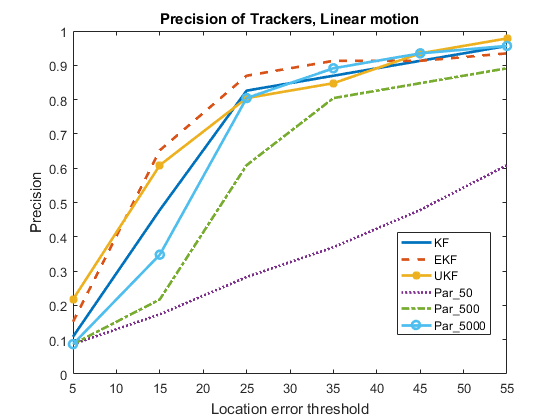
\includegraphics[width=0.5\textwidth]{Linear.png}
        \caption{\small{Precision of Trackers in Linear Motion Scenario}}
        \label{fig: linear}
 \end{figure}
 
Figure \ref{fig: linear} shows the precision of trackers in linear motion scenario. All three kinds of Kalman filters have good performance, where the trival difference among them is because the motion model is not perfectly linear, and EKF and UKF could better capture the little vibration. When the threshold becomes larger, there is no obvious difference between KF, EKF and UKF. Particle filters with 5000 and 500 particles has also good and acceptable performances. But particle filters with 50 particles has relatively poor precision, because it's hard to compute the accurate location using such few number of particles, where even little noise would sufficiently influence the result.

\begin{figure}[h]
     \centering
       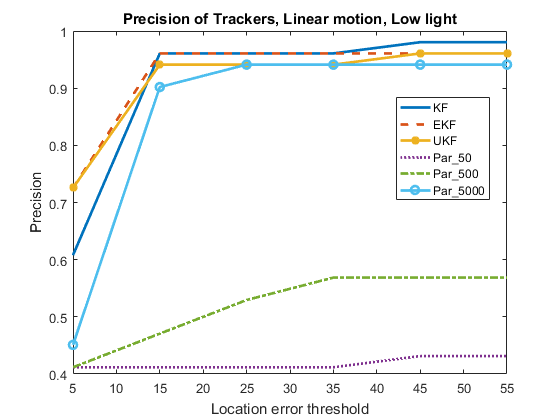
\includegraphics[width=0.5\textwidth]{Linear_Low_Light.png}
        \caption{\small{Precision of Trackers in Linear Motion and Low Light Scenario}}
        \label{fig: liner low light}
 \end{figure}
 
 \begin{figure}[h]
     \centering
       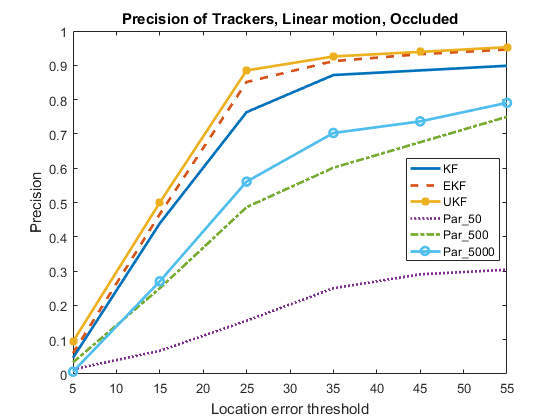
\includegraphics[width=0.5\textwidth]{Linear_Occluded.png}
        \caption{\small{Precision of Trackers in Linear Motion and Occluded Scenario}}
        \label{fig: linear occ}
 \end{figure}
 
Figure \ref{fig: liner low light} shows the results in low light scenario. We can see that the 3 Kalman filters and particle filter with 5000 particles are still robust with good precision. But the particle filters with 500 particles and 50 particles have poor performance. This is because in low light condition, it's more difficult to tell the accurate difference of color, i.e. the particle filter without enough particles have low accuracy when calculating the location.
 
 
From Figure \ref{fig: linear occ} we can see that UKF and EKF outperform KF as a result of more accurate prediction in occluded frames. While the 3 particle filters have relatively low precision. This is because when object is occluded particle filter will try to find the most similar region to target in background, i.e. the result is dominated by noise.

\begin{figure}[h]
     \centering
       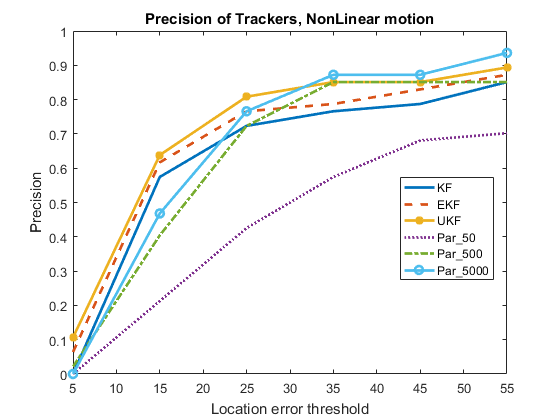
\includegraphics[width=0.5\textwidth]{Nonlinear.png}
        \caption{\small{Precision of Trackers in Nonlinear Motion Scenario}}
        \label{fig: nonlinear}
 \end{figure}
 
\begin{figure}[h]
     \centering
       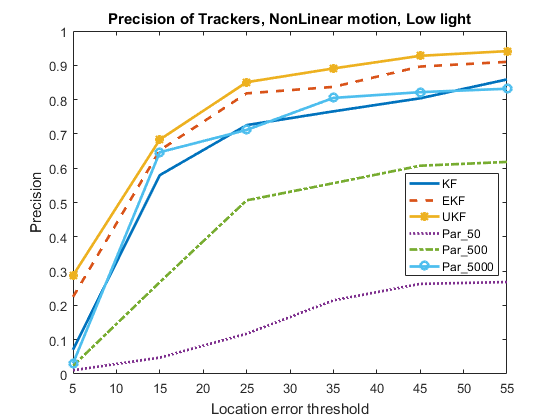
\includegraphics[width=0.5\textwidth]{Nonlinear_Low_light.png}
        \caption{\small{Precision of Trackers in Nonlinear Motion and Low Light Scenario}}
        \label{fig: nonlinear low light}
 \end{figure}
 
Figure \ref{fig: nonlinear} shows the results in nonlinear motion scenario, we can see that clearly UKF$>$EKF$>$KF, because UKF has the most accurate approximation to the nonlinear model, which confirms the hypothesis. On the other hand, particle filters with 5000 and 500 particles both have good performance.

Figure \ref{fig: nonlinear low light} shows the results in nonlinear motion and low light scenario. Compared with Fig. 6, we can see that three Kalman filters are still robust while UKF$>$EKF$>$KF. Particle filter with 5000 particles is also of good precision, even though influenced by low light inference. However, the particle filters with 500 and 50 particles have low precision because of the low light interference.

\begin{figure}[h]
     \centering
       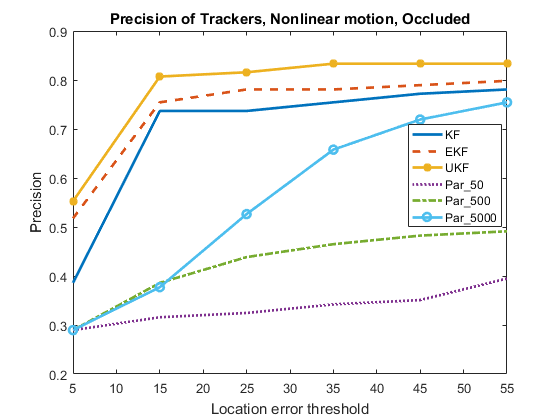
\includegraphics[width=0.5\textwidth]{Nonlinear_Occluded.png}
        \caption{\small{Precision of Trackers in Nonlinear Motion and Occluded Scenario}}
        \label{fig: nonlinear occ}
 \end{figure}

From Figure \ref{fig: nonlinear occ}, we can see that in occluded nonlinear motion scenario, it is obvious that Kalman filters are more robust than particle filters, while UKF$>$EKF$>$KF. Particle filters again have low precision because of occlusion.

%-------------------------------------------------------------------------
\section{Conclusion}

For linear motion scenario, all three Kalman filters perform well; for nonlinear motion, UKF$>$EFK$>$KF corresponding to the different precisions of approximation to the model. And all three kinds of Kalman filters have good stability in low light and occluded conditions. Particle filter needs sufficient amount of particles to ensure robustness, and it has good performance for both linear and nonlinear motion model. But once in low light or occluded conditions, the performance of particle filter declines sharply. For future work, there are many ways to improve the track precision. For example, using RGB-D camera, it is possible to reconstruct the 3-D model of target and get better tracking results \cite{ref:takimoto20163d}.

%------------------------------------------------------------------------
\bibliographystyle{IEEEtran}
\bibliography{/Users/Jingyi/Desktop/latex/finalref}


\end{document}
